\chapter{Лабораторная работа}

\section*{Цель работы}

Целью лабораторной работы является ознакомление с существующими методиками предварительной оценки параметров программного проекта и практическая оценка затрат на примере методики COCOMO (COnstructive COst MOdel — конструктивная модель стоимости).

\section*{COCOMO}

Модель COCOMO (COnstructive COst MOdel) разработана Барри Боэмом (директор USC Center for Software Engineering). Это одна из основных методик, которые применяются для оценки стоимости ПО. Среди других методик она выгодно отличается простотой расчетов.

\begin{equation}
	\begin{split}
		PM=C_1*EAF*(SIZE)^{P1} \\
		TM=C_2*(PM)^P,
	\end{split}
\end{equation}

где 
\begin{itemize}
	\item PM (Трудозатраты) -- количество человеко-месяцев;
	\item С1 -- масштабирующий коэффициент;
	\item EAF -- уточняющий фактор, характеризующий предметную область, персонал, среду и инструментарий, используемый для создания рабочих продуктов процесса;
	\item SIZE -- размер конечного продукта (кода, созданного человеком), измеряемый в исходных инструкциях (DSI, delivered source instructions), которые необходимы для реализации требуемой функциональной возможности; 
	\item P1 -- показатель степени, характеризующий экономию при больших масштабах, присущую тому процесс, который используется для создания конечного продукта; в частности, способность процесса избегать непроизводительных видов деятельности (доработок, бюрократических проволочек, накладных расходов на взаимодействие);
	\item TM (Время) -- общее количество месяцев; 
	\item C2 -- масштабирующий коэффициент для сроков исполнения; 
	\item P -- показатель степени, который характеризует инерцию и распараллеливание, присущее управлению разработкой ПО.
\end{itemize}
    
\section*{Задание 1}

Исследовать влияние атрибутов персонала (ACAP, PCAP, AEXP, LEXP) на трудоемкость (РМ) и время разработки (ТМ) для модели COCOMO. Для этого, взяв за основу любой из типов проекта (обычный, встроенный или промежуточный), получить значения PM и ТМ для одного и того же значения параметра SIZE (размера программного кода), выбрав номинальный (средний) уровень сложности продукта (CPLX) и изменяя значения характеристик персонала от очень низких до очень высоких. Повторить расчеты для проекта, предусматривающего создание продукта очень низкой и очень высокой сложности. Результаты исследований оформить графически и сделать соответствующие выводы.  

Необходимо провести сравнительный анализ атрибутов:

\begin{itemize}
	\item ACAP -- способности аналитика, 
	\item AEXP -- знание приложений, 
	\item PCAP -- способности программиста, 
	\item LEXP -- знание ЯП
\end{itemize}

для обычного, встроенного и промежуточного режима работы программы. Все замеры будут проводиться при KLOC = 100, также значения всех атрибутов, за исключением исследуемых, будут принимать значение <<номинальный>>.

Легенда:
\begin{figure}[H]
	\begin{center}
		
\includegraphics[width=0.15\textwidth]{imgs/task_1_0.png}
	\end{center}
\end{figure}

\begin{figure}[H]
	\begin{center}
		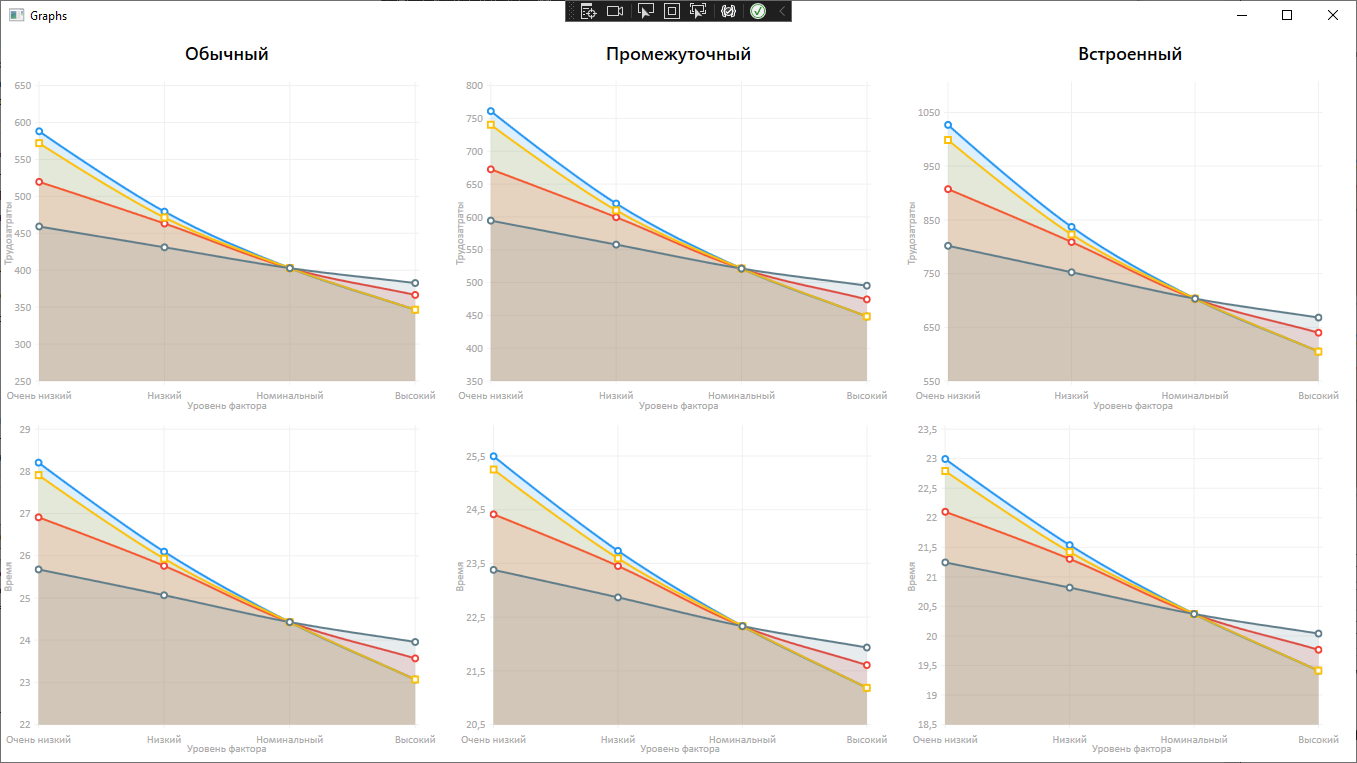
\includegraphics[width=\textwidth]{imgs/task_1_1.png}
	\end{center}
\end{figure}

Проанализировав информацию, которую отображают графики можно сделать вывод, что с ростом параметров, уменьшаются трудозатраты, что в свою очередь влияет на время реализации проекта.

Как и ожидалось, при изменении сложности проекта, форма графиков останется неизменной, а значения трудозатрат увеличивается (Обычный < Промежуточный < Встроенный), значения времени уменьшается (Обычный > Промежуточный > Встроенный).

\textit{Что больше влияет на трудоемкость и сроки реализации проекта: способности персонала или знание языка программирования и приложений?} 
На трудоёмкость и сроки значительно больше влияют способности персонала, чем знание языка программирования.

\textit{Усиливается ли влияние квалификации на трудоемкость с повышением уровня сложности продукта?}
Да

\textit{Что больше влияет на трудоемкость и время выполнения проекта при создании продукта высокой сложности: способности аналитика или способности программиста?}
Способности аналитика

\textit{Какие квалификационные характеристики выгоднее повышать, если мы хотим сократить период реализации проекта?}
Выгоднее повышать квалификацию аналитика и программистов.

\section*{Задание 2}

По предварительным оценкам размер проекта составит порядка 25 000 строк исходного кода (KLOC=25). Для реализации проекта планируется привлечь высококвалифицированную (PCAP=2) команду программистов с высоким знанием языков программирования (LEXP=1). В проекте будут использованы самые современные методы программирования (MODP=2). Так же планируется высокий уровень автоматизации процесса разработки за счет использования эффективных программных инструментов (TOOL=2). Произвести оценку по методике COCOMO для обычного режима.

Занесем настройки проекта и проанализируем результаты:

\begin{figure}[H]
	\begin{center}
		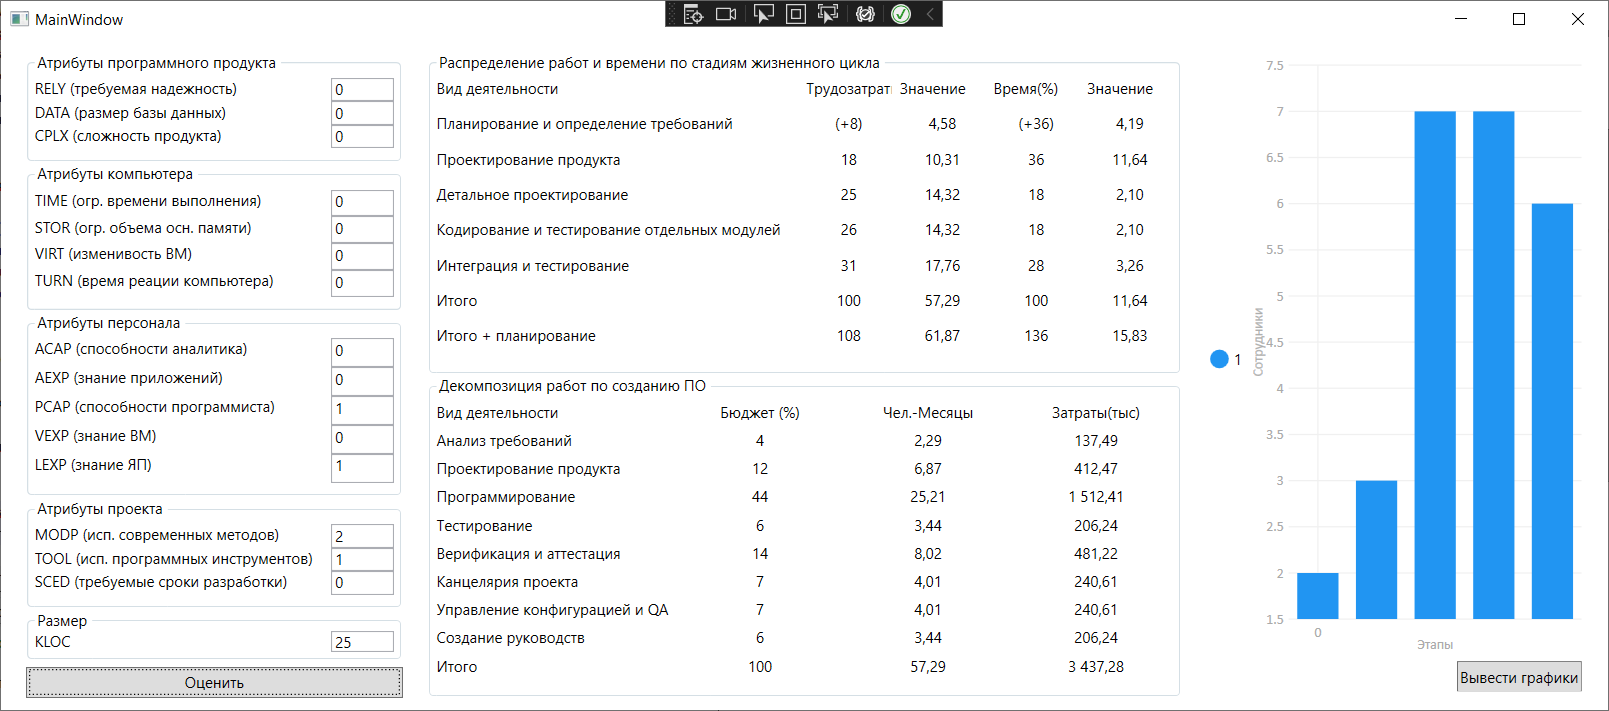
\includegraphics[width=\textwidth]{imgs/task_2_0.png}
	\end{center}
\end{figure}

Трудозатраты (с учетом доп. затрат) = 61.87

Время (с учетом доп. затрат) = 15.83

На диаграмме привлечение сотрудников видно, что 3 и 4 этапы (детальное проектирование; кодирование и тестирование) требует наибольшее количество сотрудников, равное 7.

При средней зарплате 60 тыс. р. суммарная стоимость проекта -- 3 437 280 рублей. Наибольшие затраты -- программирование.
